
\documentclass[12pt]{article}
\usepackage[margin = 1in]{geometry}
\usepackage{amsmath}
\usepackage{amssymb}
\usepackage{graphicx}
\usepackage{xcolor}
\newcommand{\ycc}[1]{\ensuremath{y_\text{#1}^\text{CC}}}
\newcommand{\yia}[1]{\ensuremath{y_\text{#1}^\text{Ia}}}
\pagestyle{empty}
\newcommand\doublebreak[0]{\par\null\par\noindent}

\begin{document}

\noindent
Dear Editor,
\par\null\par\noindent
We thank both reviewers for their time and careful consideration of our
submitted manuscript titled~\textit{Empirical Constraints on the
Nucleosynthesis of Nitrogen.}
We have taken their responses into consideration and updated the document
accordingly; changes from the submitted version are highlighted in red text.
Below you will find our separate responses to both reviewers' comments on
separate pages, with relevant excerpts of their responses in italics.
\doublebreak\null\doublebreak
Sincerely,
\doublebreak
James W. Johnson, on behalf of the authors
% \par\noindent
\newpage
\begin{center}
\textbf{Reviewer 1}
\makebox[\linewidth]{\rule{0.5\textwidth}{0.4pt}}
\end{center}
\par\noindent
We accept the valid criticisms raised by Reviewer 1.
Although a number of their concerns were addressed in the original manuscript,
their judgment has made it clear that these points were not conveyed with
sufficient clarity.
We believe the quality of the manuscript has improved significantly by
addressing these points.
We thank Reviewer 1 in advance for an additional round of consideration.
We also note that this manuscript was reviewed by another referee, and some of
the updates to the manuscript are in response to their comments.
\doublebreak
\textit{%
Indeed, I am quite surprise that the authors need to invoke galactic outflows
in the Milky Way disc, while basically ALL other teams developing GCE models
for the MW do not need to include outflows in order to reproduce the disk
properties (see, e.g., Prantzos et al. 2018; Spitoni et al. 2019, 2021; Romano
et al. 2019; Kobayashi et al. 2020, Matteucci 2021 for recent work/review).
Outflows probably develop during the early formation phases, while the much
lower SFR experienced during the secular disc evolution are unlikely to favour
the development of galactic winds.
}
\doublebreak
Indeed the community is settled on neither the proper parametrization nor the
importance of Galactic winds.
Our motivation for including them is based on empirical measurements of
deuterium and helium isotope ratios in the ISM (see Weinberg, 2017, ApJ, 851,
25 and Cooke et al., 2022, ApJ, 932, 60).
In GCE models, the abundances of primoridally produced isotopes are sensitive
to the amount of gas galaxies exchange with their surroundings.
With significant outflows, baryons processed by stars are ejected and replaced
by accretion at the primordial abundance.
Without them, these baryons remain in the ISM and their abundance continues to
increase above the primordial value.
The measured D/H abundances and the~$^3$He/$^4$He ratio in the Orion Nebula
indicate that much of the local ISM has not been processed by stars, suggesting
considerable exchange of gas between the Milky Way and its surroundings
(see discussion in Weinberg, 2017, ApJ, 851, 25 and Cooke et al., 2022, ApJ,
932, 60).
Furthermore, there is a long-standing literature on the mass-metallicity
relation that invokes mass-loaded outflows as the origin of its slope (see
Finlator \& Dave, 2008, MNRAS, 385, 2181; Peeples \& Shankar, 2011, MNRAS, 417,
2962; Chisholm, Tremonti \& Leitherer, 2018, MNRAS, 481, 1690).
Reviewer 1 points out a dearth of GCE models invoking outflows to explain the
Galactic abundance structure, constituting an absence of evidence for their
requirement.
However, this absence of evidence must not be equated to evidence of their
absence in nature.
\par
We have clarified our motivation for including outflows at the beginning of
section 2 and mentioned that we find similar conclusions when we vary the
normalization of our yields and the strength of outflows simultaneously.
We have added a statement to the introduction that we have been careful to
ensure our conclusions are not impacted by this assumption as well as other
GCE parameters.
We have also added section 4.7 to the text to summarize our results and
clarify a few of these key points.
\doublebreak
\textit{%
The discrepancies between model predictions and observations pointed out by the
authors when using ``off-the-shelf'' yields do not necessarily indicate that
the yields are inappropriate!
They may rather indicate that some of the underlying model assumptions are
incorrect...
\\
...
\\
Off-the-shelf stellar yields come from detailed studies that rest on stellar
evolution and nucleosynthesis THEORY and are anchored to many independent
observables.
GCE is not a theory (see Tinsley 1980) - it simply offers a framework within
which one can try to interpret the observations...
Before claiming that the stellar yields must follow some specific trends with
either stellar mass and/or metallicity basing on GCE arguments, one should be
sure that it is IMPOSSIBLE to adjust the free parameters of their GCE models to
reproduce average abundance trends with extant stellar yield grids.
\\
...
\\
As a matter of fact, current N yields from massive stars are found to increase
with metallicity (even a small increase as the one shown in Fig.2, left panel,
may be important when weighted with the IMF and SFH of the system...).
The finding by the authors that the yields from low- and intermediate-mass
stars by Cristallo and Ventura need an upward revision may be simply due to the
effect of the outflow, which subtracts a fraction of the newly-produced N from
the ISM. But, as already noted above, other GCE models do not need outflows at
all to explain the MW data...
}
\doublebreak
Related to the above point, we have carefully considered variations in the
strength of outflows and the normalization of yields.
As noted in the original text of section 4.2.1 and in the middle panel of Fig.
6, we can alternatively lower the strength of outflows and the normalization of
our SN yields by a factor of 3 and achieve good agreement with the Cristallo
yields.
We find similar results with the Ventura yields, but with a factor of 2.
We have adjusted the text of section 4.2.1 and added an additional model to the
middle panel of Fig. 6 to make this point more clear.
Our investigation does not constrain the absolute scale of nucleosynthetic
yields -- only ratios of yields.
We also draw Reviewer 1's attention to section 4.6, which casts the [N/O]-[O/H]
relation as an equilibrium phenomenon.
The strength of outflows (i.e., the value of~$\eta$) cancels in equation 12,
leaving behind only a ratio of yields as free parameters.
This is the primary reason why our central result -- that N yields should
increase approximately linearly with~$Z$ -- should be independent of this
assumption.
We have adjusted the text throughout to emphasize more clearly that we have
only constrained the metallicity-dependence of relative yields, and we thank
Reviewer 1 for pointing out that it was not clearly conveyed in the original
manuscript.
\doublebreak
\textit{%
A different choice of the IMF slope would impact deeply the results.
Yet, this issue is surprisingly only briefly mentioned (one sentence, p.18,
l.35) and no effort is spent to investigate quantitatively the IMF issue.
}
\doublebreak
We thank Reviewer 1 for raising the issue of the impact of the IMF.
The choice of IMF indeed impacts the computed value of~$\ycc{N}$, but it has
little impact on the ratio~$\ycc{N} / \ycc{O}$ because the massive star yields
of N and O follow similar trends with stellar mass.
We have attached two figures, both of which are variations of Fig. 2 with
steep and shallow variations of the Kroupa (2001) IMF.
When adjusting the high-mass slope to either -2.6 or -2.0, factor of~$\sim$2
changes in~$\ycc{N}$ are found, but the inferred values of [N/O]$_\text{CC}$
are largely unaffected.
\par
Variations in the IMF should not impact our conclusions regarding AGB star
enrichment either.
Changing the IMF would alter the effective DTD through adjusting the relative
numbers of stars of different masses.
While we advocate for a~$\sim$250 Myr restitution delay of N production, this
value is not tightly constrained as the impact of the DTD on gas-phase
abundances is negligible and the impact on stellar abundances is only
noticeable in the limiting cases discussed in section 4.4 in relation to Fig. 9.
We have updated the text in section 2.1 the clarify this point and included a
statement in the new section 4.7 to this effect.
\doublebreak
\textit{%
It would be helpful to analyse the evolution of C as well and see if the
proposed corrections to the published N yields lead to a coherent revision of
the C yields, since the production paths of these two elements in stars are
intimately related...
}
\doublebreak
We wholeheartedly agree!
We have a student working on exactly this project, and he is currently writing
the paper.
\doublebreak
\textit{%
From Fig.1 it is seen that most data sets deviate markedly from the [N/O]-[O/H]
trend suggested by Dopita et al. at high metallicities. This is very clear for
the Pilyugin and CHAOS data, but also Belfiore shows a steeply increasing trend
of [N/O] at the highest [O/H] that is not seen in Dopita's trend. May this
affect some of the conclusions? It should also be stated if the ratios are
normalized to the same solar reference.
}
\doublebreak
Indeed, we would infer that N yields should scale approximately super-linearly
with metallicity if we had adopted one of these steeper observational
benchmarks.
We have added a statement to this effect in the conclusion as well as in the
new section 4.7.
\doublebreak
\textit{%
The authors use MESA stellar evolutionary models to correct N abundances in
giant stars from APOGEE. For the sake of consistency, they could have also
adopted stellar yields obtained from MESA tracks (e.g. Battino et al. 2021, and
refs therein).
}
\doublebreak
We thank Reviewer 1 for drawing our attention to Battino et al. (2021).
However, these yields are only sampled at two stellar masses and two
significantly sub-solar metallicities.
This is unfortunately not densely sampled enough to warrant investigation in
the present manuscript as the abundance evolution will be highly dependent on
how yields are extrapolated to the full stellar mass range and -- more
importantly -- to metallicities appropriate for the Milky Way.
\doublebreak
\textit{%
It is unclear how the authors treat the masses of N present at star birth that
are ejected without any nuclear processing. It seems that their description only
refer to newly-produced elements in stars... Regarding their footnote 7, the
yields of Fe for the Ventura's stars should be computed as (m\_ini - m\_remn)
X\_Fe,ini, where m\_ini, m\_remn, and X\_Fe,ini are, respectively, the initial
mass of the star, the mass of the remnant, and the initial Fe abundance. So, no
need to adopt Fe yields from other studies...
}
\doublebreak
We thank Reviewer 1 for pointing out that this detail was not included in the
submitted manuscript.
We have added a reference to our previous papers as well as the VICE science
documentation which discuss the treatment of previous nucleosynthetic material
returning to the ISM from ejected stellar envelopes.
The formalism they allude to is exactly how this recycling is handled.
While the other tables included in this study find slightly negative Fe yields,
this net destruction is negligible.
We have redacted footnote 7 and modified the text in section 2.2 to simply
state that we do not discuss these yields for this reason.
\doublebreak
\textit{%
Some important references are missing. For instance, when it is stated (p.10)
that "The separation of these evolutionary tracks contests the popular
interpretation that the [N/O]-[O/H] relation arises as an evolutionary
sequence..." the seminal paper by Chiappini et al. (2003) must be quoted (see
their figure 13, and the relevant discussion in their paper). Also, the work of
Tinsley (1979) should be acknowledged when noticing that elements with similar
"restitution delays" share a similar behaviour (p.14).
}
\doublebreak
We have added these references in sections 4.1 and 4.4.

\newpage
\begin{figure*}[!h]
\centering
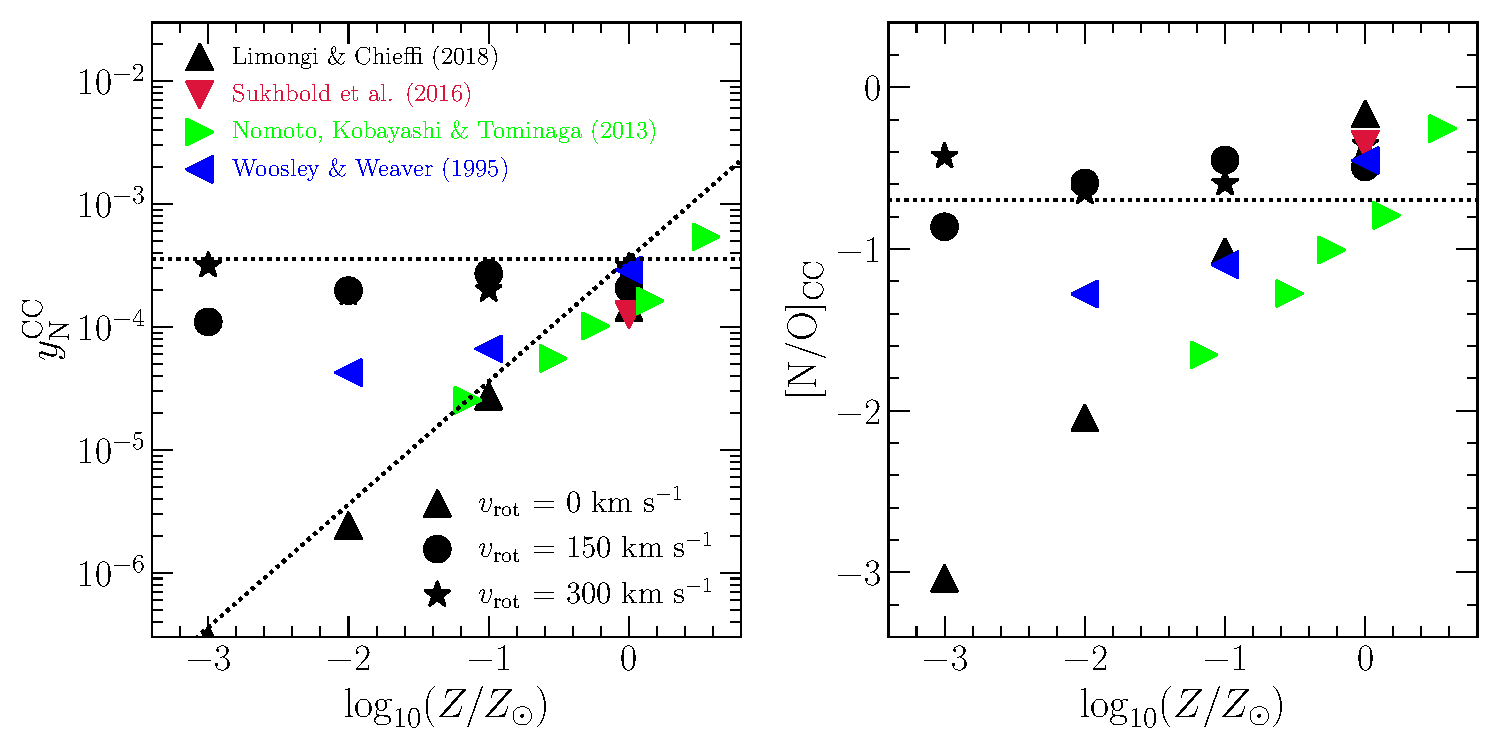
\includegraphics[scale = 0.6]{n_cc_yields_steep.pdf}
\caption{
A version of Fig. 2 in the manuscript in which the slope at the high mass end
of the Kroupa (2001) IMF is modified from -2.3 to -2.6.
}
\end{figure*}
\begin{figure*}[!h]
\centering
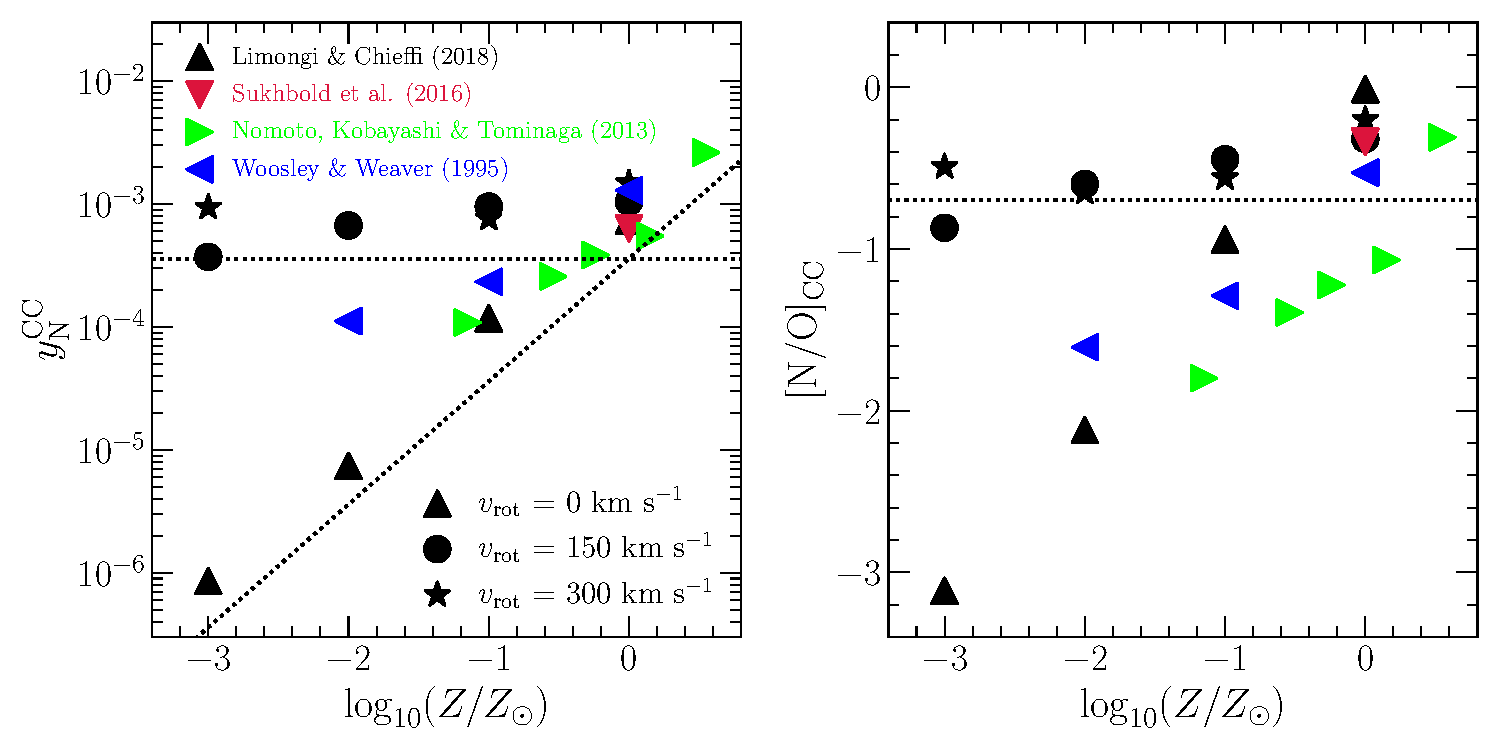
\includegraphics[scale = 0.6]{n_cc_yields_shallow.pdf}
\caption{
The same as Figure 1 above, but for a shallow IMF with a high mass slope of
-2.0.
}
\end{figure*}

\newpage
\begin{center}
\textbf{Reviewer 2}
\makebox[\linewidth]{\rule{0.5\textwidth}{0.4pt}}
\end{center}
\par\noindent
We thank Reviewer 2 for their comments.
We have adjusted the manuscript accordingly and believe that the quality of the
manuscript has improved markedly.
We thank them in advance for an additional round of considerations.
We also note that this manuscript was reviewed by another referee, and some of
the updates to the manuscript are in response to their comments.
\doublebreak
\textit{%
It is true that the present
work is based on a number of assumptions, which may affect the robustness of the
conclusions reached. For this reason the authors must declare this partial
weakness of the work in the abstract, warning the reader against possible
over-interpretations of the conclusions reached.
}
\doublebreak
It is indeed important to raise the concern about model-dependence.
We have adjusted the abstract accordingly.
\doublebreak
\textit{%
1) In the text I see that the authors refer to thermal pulsations instead of
thermal pulses (e.g. page 2, r.c., line 45). Please change
}
\doublebreak
Corrected.
\doublebreak
\textit{%
2) In the introduction the authors comment on the differences among AGB models
from various groups, invoking the treatment of microphysics as possible reason
for that.
Indeed the differences are mostly related to convection and mass loss, which is
more a matter if macrophysics. Please correct
}
We have simply redacted this term.
\doublebreak
\textit{%
3) Would the authors explain why the approach by Vincenzo et al (second to last
paragraph of the introduction) should work for external galaxies too?
}
\doublebreak
We compare only the stellar abundances of our model against the Vincenzo et al.
(2021) measurements.
While Dopita et al. (2016) present a calibration method for external galaxies,
the sample in Fig. 1 is their calibration sample from local stars and HII
regions, and Vincenzo et al. (2021) find good agreement with those data.
The reason for taking Dopita et al. (2016) is simply that they are
representative of the overall trend.
This and the apparent universality of the trend indicate that our analysis
should extend to external galaxies.
The inferred metallicity dependence of N yields would be slightly super-linear
if we had adopted one of the steeper [N/O]-[O/H] relations from Fig. 1.
We have added a statement to this effect to the conclusion and in the new
section 4.7 summarizing our results.
\doublebreak
\textit{%
Footnote 2 can be deleted. No need to give these details.
}
Redacted.
\doublebreak
\textit{%
In section 2.1 tha authors use the term "yield" for the quantities given by
equation 1.
This term is commonly used for gas or dust mass from single stars. Please give
an alternative term here
}
\doublebreak
There are a number of GCE papers that use the term yield to refer to chemical
yields from whole populations of stars.
Respectfully, we elect to retain our current nomenclature to remain consistent
with this literature.
\doublebreak
\textit{%
6) The authors should add a short paragraph in section 2.1, to stress that some
rotation of massive stars is required to reproduce the N patterns, although it
is not possible to quantify tightly the rotation rate, based on the present
observational evidence.
}
\doublebreak
We thank Reviewer 2 for this suggestion.
It is already discussed in relatively great detail that rotation is required to
reproduce N abundance patterns, particularly at low metallicity.
We have however added a statement to the second to last paragraph of section
2.1.
\doublebreak
\textit{%
7) When discussing the differences among AGB models (section 2.2, page 5, r.c.,
lines 45-50)
I ask the authors to mention some works where these differences are extensively
discussed and commented: the review by Karakas \& Lattanzio (2014), the papers
Ventura et al. (2018, MNRAS 475, 2282) and Ventura et al. (2016, MNRAS, 457,
1456).
\doublebreak
8) Citations to HBB are lacking. Please add some works e.g. by Sackmann \&
Boothroyd and also Blocker \& Schoenberner
\doublebreak
9) Page 6, second to last paragraph. Note that among the reasons for the
differences
between C11+C15 and the other modellers, the discrepancies among the
temperatures at
the base of the envelope are the dominant ones.
}
\doublebreak
We thank Reviewer 2 for directing our attention to these references and
discussion points.
We have adjusted the text accordingly.
\doublebreak
\textit{%
10) I ask the authors to shorten the discussion on the solar metallicity at the
beginning of page 7. We do not need all the details given
\doublebreak
11) page 7, l.c., line 14. Not only the description of more massive AGB stars are
touched by the description of the opacities. Please change
}
\doublebreak
We have adjusted this text to make it more clear which metallicities and which
masses we are referring to in each sentence.
We however elect to retain the discussion of the solar metallicity as its
downward revision with time plays an important role in the differences between
the Karakas yields from 2010 at Z = 0.02 and from 2016/2018 at Z = 0.014.
\doublebreak
\textit{%
12) Section 3 provides a detailed description of the chemical evolution model
adopted.
Please keep the main points here, and move the rest to an appendix.
}
\doublebreak
We thank Reviewer 2 for letting us know that section 3 is somewhat lengthy.
Unfortunately, many of these details are relevant later in the paper.
We have done our best to keep the summary of the model concise, but the full
description in Johnson et al. (2021) is nearly 8 pages.
We therefore elect to keep section 3 as is.
\doublebreak
\textit{%
13) The ylabel of the left panel of Fig. 4 is unclear. Please change
}
Adjusted -- the new label is simply ``IMF-weighted N Yields.''
\doublebreak
\textit{%
14) Section 4.2 can be substantially shortened.
}
Reviewer 1 actually raised concerns about the content of section 4.2,
particularly 4.2.1, which discusses our central result.
We have made adjustments to this text, which are approximately length-neutral.
\doublebreak
\textit{%
15) In the conclusions, please comment again on the uncertainties (see my first
comment above)
}
\doublebreak
As with the above point, this is a good suggestion.
We have made a handful of adjustments to the conclusions.



\end{document}































